\documentclass{article}
\usepackage[utf8]{inputenc}
\usepackage{graphicx}
\usepackage{geometry}
\geometry{a4paper, total={16cm, 24cm}, top=2cm}
\usepackage{amsmath}
\usepackage{blindtext}
\graphicspath{ {img/} }
\usepackage{listings}
\usepackage{color}
\usepackage{siunitx}
\usepackage{hyperref}
\hypersetup{
    colorlinks=true,
    linkcolor=blue,
    filecolor=magenta,      
    urlcolor=cyan,
    }
\definecolor{dkgreen}{rgb}{0,0.6,0}
\definecolor{gray}{rgb}{0.5,0.5,0.5}
\definecolor{mauve}{rgb}{0.58,0,0.82}
\renewcommand{\thesubsection}{(\alph{subsection})}

\lstset{ %frame=tb,
  language=C,
  aboveskip=3mm,
  belowskip=3mm,
  showstringspaces=false,
  columns=flexible,
  numbers=left,
  basicstyle={\small\ttfamily},
  numberstyle=\tiny\color{gray},
  keywordstyle=\color{blue},
  commentstyle=\color{dkgreen},
  stringstyle=\color{mauve},
  breaklines=true,
  breakatwhitespace=true,
  tabsize=3  
}


\title{Week 7 Programming Assignment}
\author{Steffen Petersen | au722120}
\date{October 20th 2022}

\begin{document}
%\tableofcontents

\maketitle
\vspace{5pt}
\noindent Here is the link for my repository, in which you will find all the edited code files and such.\\
\url{https://github.com/Aarhus-University-ECE/assignment-7-SirQuacc}
\section{}
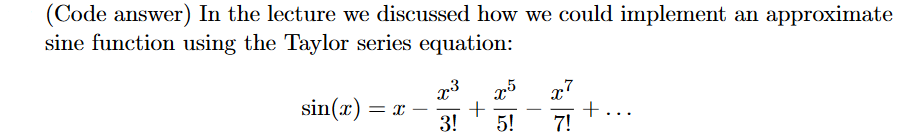
\includegraphics[width=\linewidth, keepaspectratio=true]{task1}
\subsection{}
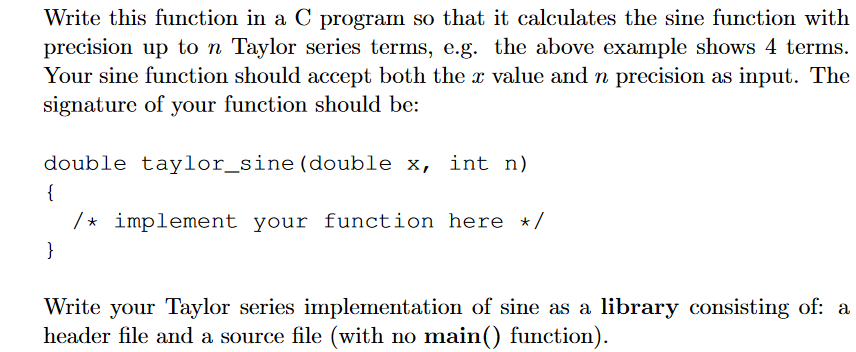
\includegraphics[width=\linewidth, keepaspectratio=true]{task1a}
Everything can be found in the repository, respectively in the /include/taylor\_sine.h file and \\/src/taylor\_sine.c file, but below is also
the standalone taylor\_sine function.

\begin{lstlisting}
    double taylor_sine(double x, int n)
    {
        double sine = 0; //Initialize variable to return
        int swapCount = 0; //Keep track of whether to add or subtract from previous result in the for loop.
        for (int i = 1; swapCount <= n; i+=2){
            if(swapCount%2 == 0){ //even swapCount, when the next bit is added to the previous
                sine += pow(x, i)/factorial(i); //Culcalation based on the taylor sine formula
                swapCount++;
            }
            else{ //uneven swapCount, when the next bit is subtracted from the previous
                sine -= pow(x, i)/factorial(i);
                swapCount++;
            }
        }
        return sine;
    }
\end{lstlisting}

\subsection{}
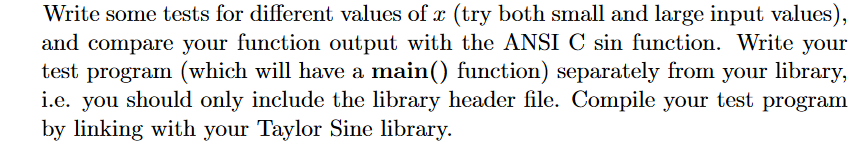
\includegraphics[width=\linewidth, keepaspectratio=true]{task1b}
This has been done in the /src/main.cpp as the main() function, where it runs through a series of input x values with
a series of different precision values.

\subsection{}
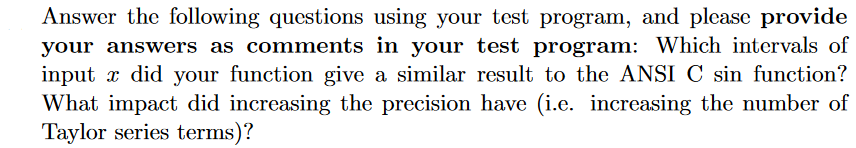
\includegraphics[width=\linewidth, keepaspectratio=true]{task1c}
Generally speaking the lower values of x are easier to get right, even with lower precision, and when the x values are higher, it's necessary
to have a higher precision, before it becomes a reasonably valid result.\\
That said, with too high x-values, my function at least, also appears to run into overflow problems, meaning results are way out of wack compared to
the sin() function from the standard math.h library.\\
And as expected with too high precision, meaning lots of taylor series terms, it will also run into problems, and the result 
will output an error.


\section{}
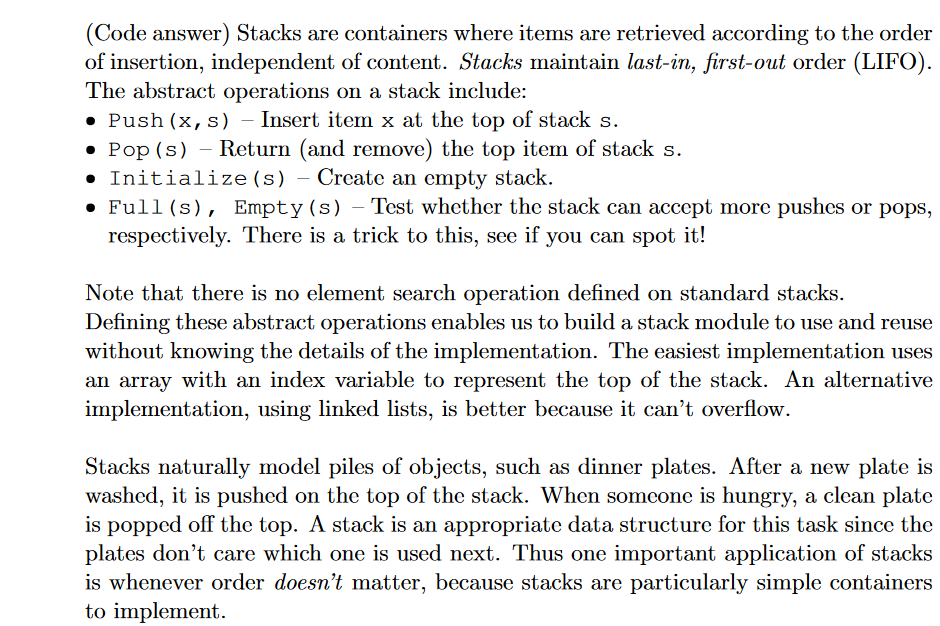
\includegraphics[width=\linewidth, keepaspectratio=true]{task2}
\subsection{}

\includegraphics[width=\linewidth, keepaspectratio=true]{task2a}
The implementation can be seen in the repository, as a combination of the stack.c and stack.h files in the /src and /include directories respectively.

\subsection{}
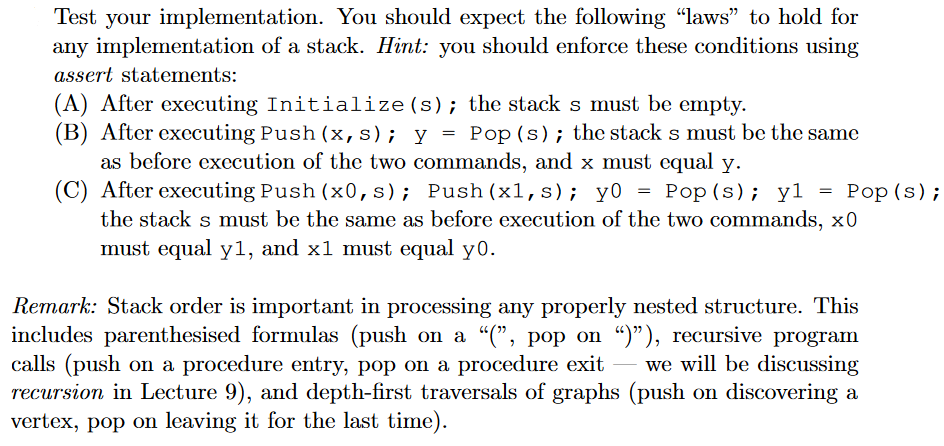
\includegraphics[width=\linewidth, keepaspectratio=true]{task2b} 
These tests are all present in /tests/src/tests.cpp and have been run with CMake to confirm.


\end{document}